%%%%%%%%%%%%%%%%%%%%%%%%%%%%%%%%%%%%%%%%%%%%%%%
%%% Template for lab reports used at STIMA
%%%%%%%%%%%%%%%%%%%%%%%%%%%%%%%%%%%%%%%%%%%%%%%

%%%%%%%%%%%%%%%%%%%%%%%%%%%%%% Sets the document class for the document
% Openany is added to remove the book style of starting every new chapter on an odd page (not needed for reports)
\documentclass[10pt,english, openany]{book}

%%%%%%%%%%%%%%%%%%%%%%%%%%%%%% Loading packages that alter the style
\usepackage[]{graphicx}
\usepackage[]{color}
\usepackage{alltt}
\usepackage[T1]{fontenc}
\usepackage[utf8]{inputenc}
\setcounter{secnumdepth}{3}
\setcounter{tocdepth}{3}
\setlength{\parskip}{\smallskipamount}
\setlength{\parindent}{0pt}
\usepackage{multicol}

% Set page margins
\usepackage[top=100pt,bottom=100pt,left=68pt,right=66pt]{geometry}

% Package used for placeholder text
\usepackage{lipsum}

% Prevents LaTeX from filling out a page to the bottom
\raggedbottom

% Adding both languages
\usepackage[english, italian]{babel}

% All page numbers positioned at the bottom of the page
\usepackage{fancyhdr}
\fancyhf{} % clear all header and footers
\fancyfoot[C]{\thepage}
\renewcommand{\headrulewidth}{0pt} % remove the header rule
\pagestyle{fancy}

% Changes the style of chapter headings
\usepackage{titlesec}
\titleformat{\chapter}
   {\normalfont\LARGE\bfseries}{\thechapter.}{1em}{}
% Change distance between chapter header and text
\titlespacing{\chapter}{0pt}{50pt}{2\baselineskip}

% Adds table captions above the table per default
\usepackage{float}
\floatstyle{plaintop}
\restylefloat{table}

% Adds space between caption and table
\usepackage[tableposition=top]{caption}

% Adds hyperlinks to references and ToC
\usepackage{hyperref}
\hypersetup{hidelinks,linkcolor = black} % Changes the link color to black and hides the hideous red border that usually is created

% If multiple images are to be added, a folder (path) with all the images can be added here 
\graphicspath{ {Figures/} }

% Separates the first part of the report/thesis in Roman numerals
\frontmatter


%%%%%%%%%%%%%%%%%%%%%%%%%%%%%% Starts the document
\begin{document}

%%% Selects the language to be used for the first couple of pages
\selectlanguage{english}


\mainmatter


\begin{centering}

	{\LARGE \textbf{Gebze Technical University}} \\
	{\LARGE \textbf{Computer Engineering}} \\
	    \vspace{2.0cm}
	    
\begin{figure}[htp]
    \centering
    
\includegraphics[width=5cm]{gtu_logo.png}
    
\end{figure}	    
	    
	    \vspace{2.0cm}
	    
	{\LARGE \textbf{System Programming}} \\
	{\LARGE \textbf{CSE344 – 2021}} \\
	    \vspace{3.0cm}
	
	{\LARGE \textbf{MIDTERM-REPORT}} \\
		\vspace{3.0cm}

	{\LARGE \textbf{Yusuf Abdullah ARSLANALP}} \\
	{\LARGE \textbf{151044046}} \\
	    %\vspace{3.0cm}


\end{centering}



\newpage


\section{How I Solved This Problem}
I used 7 semaphore to solve the problem. Semaphores are as follows:

\vspace{0.5cm}

\begin{figure}[htp]
    \centering
    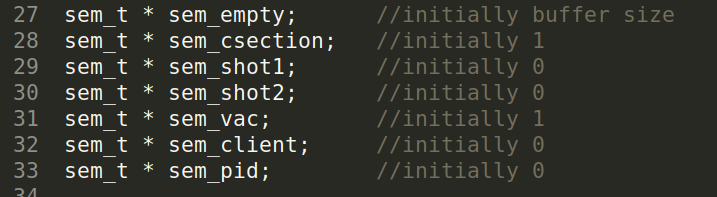
\includegraphics[width=15cm]{sems.png}
    
\end{figure}

The pseudocode for nurse-vaccinator synchronization is as follows:

\begin{figure}[htp]
    \centering
    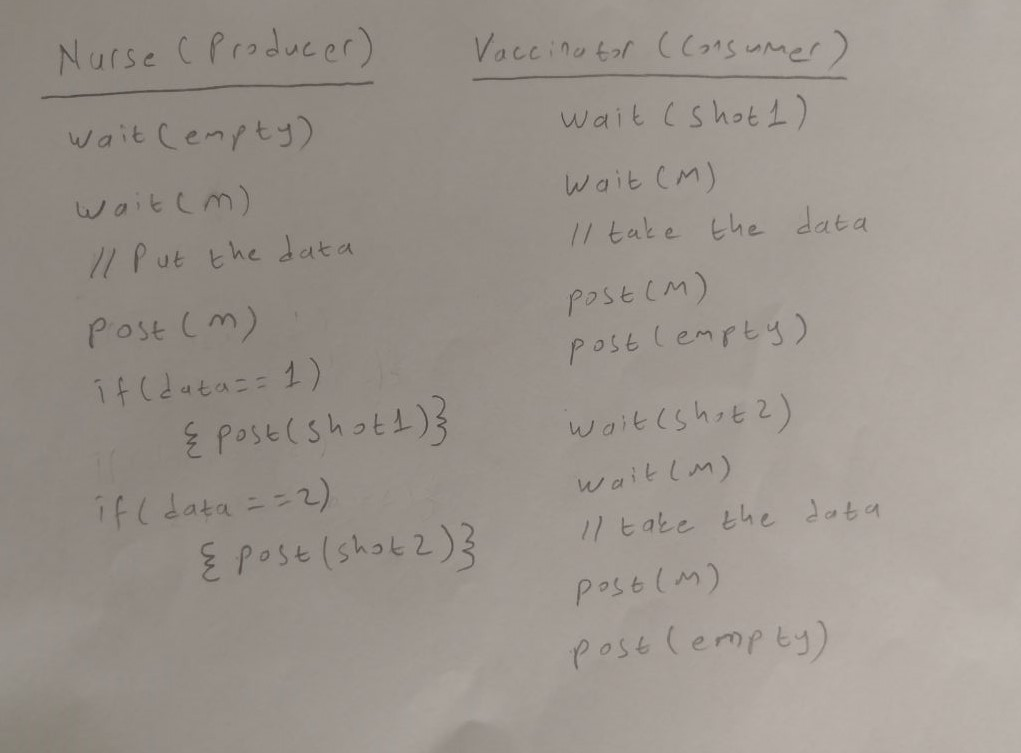
\includegraphics[width=15cm]{nurse-vaccinator.jpg}
    
\end{figure}

\newpage

The pseudocode for nurse-vaccinator synchronization is as follows:

\begin{figure}[htp]
    \centering
    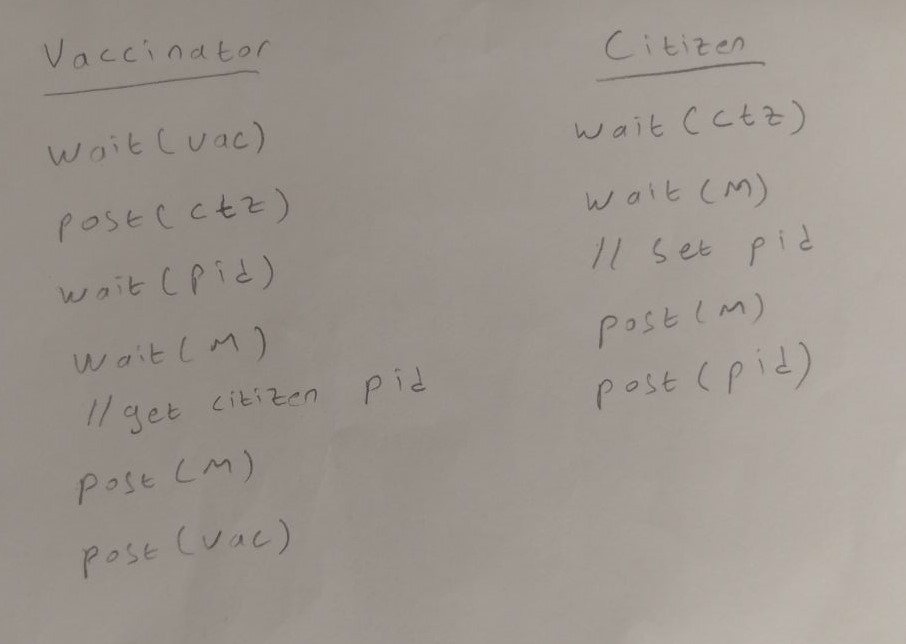
\includegraphics[width=15cm]{vaccinator-citizen.jpg}
    
\end{figure}


\section{To solve this problem in addition to semaphores I used:}

\begin{itemize}
  \item named fifo
  \item Signal
  \item Named shared memory
\end{itemize}
\section{Which requirements I achieved}

\begin{itemize}
  \item I Protect the buffer against underflow and overflow
  \item No race condition for the buffer
  \item Input file is read sequentially.
  \item When CTRL-C pressed all processes terminated. And all resources are given back to the system.
  \item I used only 7 semaphore
  \item No warning with -Wall flag
  \item If the required command line arguments are missing/invalid, The program prints usage information and exit.
  \item The report prepeared via latex. (latex folder is in the homework)
  \item No zombie processes
  \item No busy waiting. No sleep.
  \item The make file only compiles the program.
  \item No memory leaks.
\end{itemize}


\begin{figure}[htp]
    \centering
    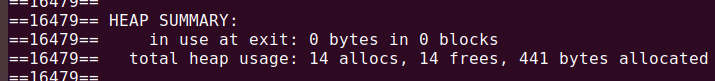
\includegraphics[width=18cm]{no-leak.png}
    
\end{figure}



\end{document}
